\section{Day 13: Connectivity (Oct. 15, 2024)}
Outfit of the day! red shirt!!!
\begin{figure}[h]
    \centering
    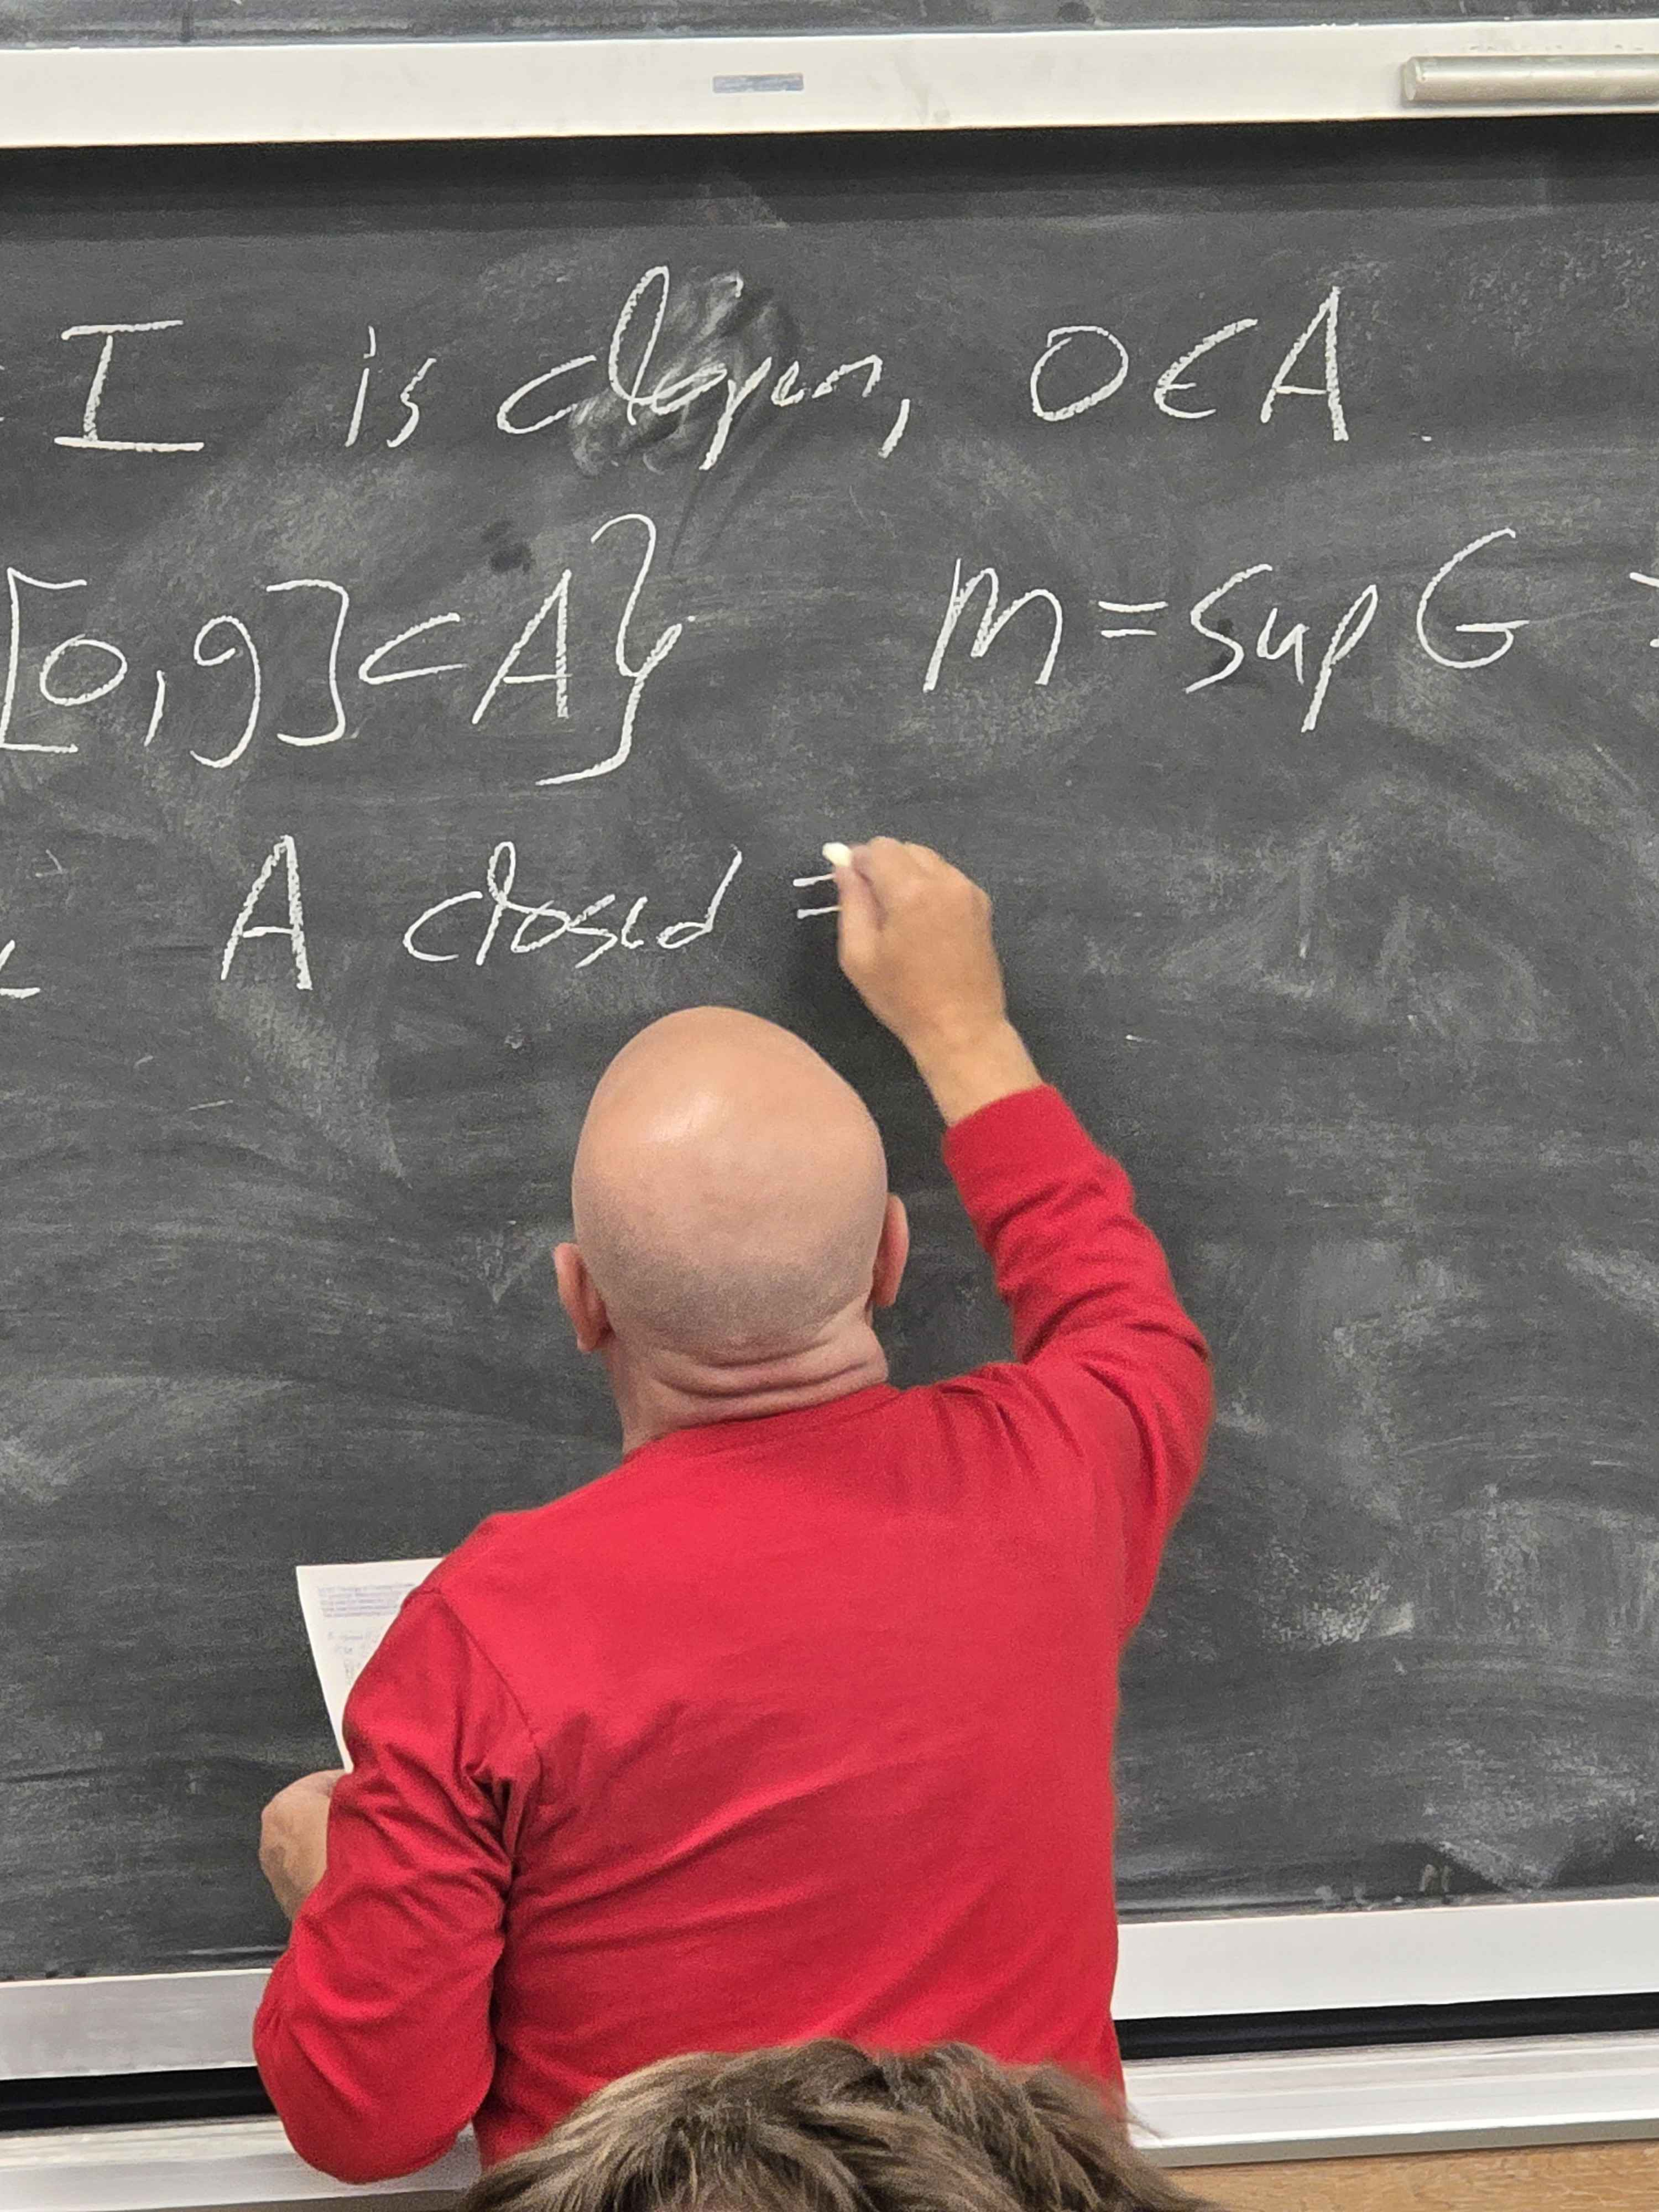
\includegraphics[scale=0.1]{MAT327 Notes/Dror Shirts/dror day 13 shirt.jpg}
\end{figure}

\noindent Term test information is given \href{https://drorbn.net/AcademicPensieve/Classes/24-327-Topology/TTInfo.pdf}{here}. Recap!
Consider the function space $\RR^\RR = \SL(\RR, \RR)$, aka all functions $f : \RR \to \RR$. We claim that $\RR^\RR$ is \textit{not} metrizable. Consider the subset $A \subset \RR^\RR$ where $A$ is given by
\[ A = \{f : \RR \to \RR \mid \abs{\mathrm{supp} f} < \infty \}. \]
We make the following claims:
\begin{enumerate}[label=(\alph*)]
    \item The function $\overline{1}(x) = 1$ is in the closure of $A$, but
    \item $\overline{1} \not\in \mathrm{scl}(A)$. This means that $\RR^\RR_\mathrm{cyl}$ is not metrizable.
\end{enumerate}
We prove the first claim. $A$ intersects every open set containing non-empty open set, i.e.
\[ U = \prod_{\alpha \in \RR} U_\alpha, \] 
where we see that $U_\alpha = \RR$ for all but finitely many indices; let these indices be given by $\alpha_1, \dots, \alpha_n$. Pick $y_i \in U_{\alpha_i}$, and let $f(\alpha_i) = y_i$, and $f(\alpha) = 0$ if $\alpha \neq \alpha_i$ for some $i$. Then $\mathrm{supp} f \subset \{\alpha_i\}$, so $f \in A$, and also $f \in U$ as $f(\alpha) \in U_\alpha$ for all $\alpha$. Indeed, this holds over the indices $\alpha_1, \dots, \alpha_n$, and for the rest there is nothing to check.
\medskip\newline
For the second claim, suppose $f_n \to \overline{1}$, and $f_n \in A$. Then the support of $f_n$ is finite, and so the union of the supports of all $f_i$ is also countable. Then choose $\alpha \not\in \bigcup_{n=1}^{\infty} \mathrm{supp}(f_n)$, meaning $f_n(\alpha) = 0$ for all $\alpha$. Then $U = \prod U_\beta$, where $U_\beta$ can be picked as $(\frac{1}{2}, \frac{3}{2})$ if $\alpha = \beta$, and $\RR$ otherwise. Then $U$ is open, $\overline{1} \in U$, none of $f_n$ are in $U$, as $f_n(\alpha) = 0 \not\in U_\alpha$. \qed
\medskip\newline
\noindent We now return to connectedness. If $X$ is connected, then $X$ is not empty, and has no clopen subsets aside from $\emptyset$ and $X$.
\begin{simplethm}
    Let $X$ be connected, and consider a continuous function $f : X \to \RR$, where $f(x_0) < 0, f(x_1) > 0$ implies that there exists $x$ such that $f(x) = 0$.
\end{simplethm}
\noindent Suppose that there does not exist $x$ such that $f(x) = 0$; then we have that $X = f^{-1}((-\infty, 0)) \cup f^{-1}((0, \infty))$. Each of the pre-images are open, since they are the pre-images of open sets; they are also nonempty, since $x_0$ belongs to the former and $x_1$ belongs to the latter. Since there does not exist $x$ such that $f(x) = 0$, their intersection is empty, and so have a non-trivial separation of $X$, contradicting the connectiveness of $X$. \qed
\begin{simplethm}
    $I = [0, 1]$ is connected.
\end{simplethm}
\noindent Assume $A \subset I$ is clopen, and $0 \in A$. Let $G := \{g \in I \mid [0, g] \subset A\}$, and let $m = \sup G > 0$. Then $m = 1$; if not, we would have $m < 1$: using that $A$ is closed, we have $m \in A$. Moreover, since $A$ is open, there exists $\eps > 0$ such that $(m - \eps, m + \eps) \subset A$, and then $m + \frac{\eps}{2} \in G$, meaning $m \geq m + \frac{\eps}{2}$, which is obviously untrue. It remains to show that $1 \in G$. Indeed, $A$ is closed, and so $G \subset A$, meaning $1 = m = \sup G \in \overline{G} \subset \overline{A} = A$. But $A$ is open, and so for some $\eps > 0$, $(1 - \eps, 1] \in A$. Pick some $g \in G$ such that $g > 1 - \eps$. Then $[0, 1] = [0, g] \cup (1 - \eps, 1] \subset A$. The former is in $A$, since $g \in G$, and the latter is in $A$ by choice. \qed
\begin{simpleclaim}
    A continuous image of a connected set is connected; e.g., $[a, b] = f([0, 1])$.
\end{simpleclaim}
\noindent Suppose $A$ is a non-trivial clopen in $Y$; then $f^{-1}(A)$ is a non-trivial clopen in $X$.
\begin{simpleclaim}
    If, for all indices $\alpha$, the subsets $A_\alpha \subset X$ is connected, and $\bigcap A_\alpha \neq \emptyset$, then $\bigcup A_\alpha$ is connected.
\end{simpleclaim}
\noindent Suppose $B \subset \bigcup A_\alpha$ is clopen and non-empty. Then, for some $\alpha_0$, $B \cap A_{\alpha_0} \neq \emptyset$. But $A_{\alpha_0}$ is connected, so $B \supset A_{\alpha{0}}$, meaning $B \supset \bigcap A_|alpha \neq \emptyset$, and so for all indices $\alpha_i$, $B \cap A_{\alpha_i} \neq \emptyset$, but $A_{\alpha_1}$ is connected, and so $B \cap A_{\alpha_1} = A_{\alpha_1}$, so for all $\alpha$, $B \supset A_\alpha$, so $B \supset \bigcup A_\alpha$. \qed
\medskip\newline
\noindent As a corollary, $[a, b), (a, \infty), (-\infty, a)$ are connected. To prove this, write them as a union of closed intervals, etc...